\part{Internship Contribution}

\chapter{Global Near-optimal Solution for Path Planning}
\lipsum[1]
\section{Description of the Problem}

\chapter{Algorithmic Approach}
\lipsum[1]
\newpage
\section{Representation of the optimization problem}

\subsection{Optimizers}

There is a variety of numerical optimization packages implemented in many different programming languages available for solving optimization problems \cite{pyopt-paper}. Each of them may have their own way of defining the optimization problem and may or may not support specific kinds of constraints (equations, inequations or boundaries).

For the initial implementation written in python two packages stood out as good, easy-to-use options for solving the constrained optimization problem that models the planning motion task.

\textbf{Scipy} is a vast open-source scientific package based on python that happens to have a minimization module. Within this module many minimization methods can be found. For this specific optimization problem, only the method SLSPQ was appropriate. It was the only one to handle constrained minimization where the constraints could be equations as well as inequations.

\textbf{pyOpt} is a much smaller ecosystem than Scipy that is specialized in optimization. It gathers many different numerical optimization algorithms some of them free and some licensed. Again, among all of them there were only a few suitable for this problem which were also free: SLSQP (same as the one implemented within Sicpy), PSQP and ALGENCAN.

SLSQP and PSQP are both SQP (for sequential quadratic programming) methods. A SQP method attempts to solve a nonlinearly constrained optimization problem where the object function and the constraints are twice continuously differentiable. It does so by modeling the object function ($\min f(x)$) at the current iterate $x_k$ by a quadratic programming subproblem and using the minimizer of this subproblem to define a new iterate $x_{k+1}$ \cite{Nocedal}.

The ALGENCAN method\todo[inline, size=\tiny]{describe algecan}

% Following we present briefly these three methods:

% \begin{itemize}

% \item SLSQP: optimizer is a sequential least squares programming algorithm which uses the Han–Powell quasi–Newton method with a BFGS update of the B–matrix and an L1–test function in the step–length algorithm. The optimizer uses a slightly modified version of Lawson and Hanson’s NNLS nonlinear least-squares solver

% \item PSQP
% \item ALGENCAN
% \end{itemize}

\paragraph{Cost function} chosen was the $(t_{final}-t_{initial})^2$. This $J$ value yields to a convergence while the using only the difference does not (for a given accuracy). Also there is the Hessian problem: slsqp try to invert the Hessian matrix which will be virtually zero for a linear cost function (if zero the error \texttt{Singular matrix C in LSQ subproblem (Exit mode 6)} is shown when using \texttt{scipy} optimization module)

The optimization problem for the first implementation:

% \begin{equation}
% 	\underset{(t_{final},C_0,\dotsc,C_{d+n_{knot}-2})}{\mathrm{min}} J = \int_{t_{initial}}^{t_{final}}dt
% \end{equation}

\begin{equation}
	\underset{(t_{final},C_0,\dotsc,C_{d+n_{knot}-2})}{\mathrm{min}} J = (t_{final}-t_{initial})^{2}
\end{equation}

under the following constraints $\forall k \in \{0,\dotsc,N_s -1\}$:
\begin{equation}%\label{eq:sysr4}
\left\lbrace\begin{array}{lcl}
	\varphi_1(z(t_{initial}),\dotsc,z^{(l-1)}(t_{initial})) & = & q_{initial}\\
    \varphi_1(z(t_{final}),\dotsc,z^{(l-1)}(t_{final})) & = & q_{final}\\
    \varphi_2(z(t_{initial}),\dotsc,z^{(l)}(t_{initial})) & = & u_{initial}\\
    \varphi_2(z(t_{final}),\dotsc,z^{(l)}(t_{final}))& = & u_{final}\\
    \varphi_2(z(t_k),\dotsc,z^{(l)}(t_k)) &\in& \mathcal{U}\\
    d_{O_m}(t_k) &\geq& \rho + r_m,\quad \forall O_m \in \mathcal{Q}_{occupied}
\end{array}\right.
\end{equation}

\paragraph{Practical stuff for implementation}

$q \in \R^n$ and $u \in \R^m$. $N_s$ number of time steps used when computing the problem.

Number of equations: $2n + 2m$

Number of inequations: $N_s(m+\mathrm{card}(\mathcal{Q}_{occupied}))$

\paragraph{OPTIMIZERS}\footnote{CFSQP, SNOPT, NLPQL and FSQP are licensed} CFSQP is the name of the solver used by Defoort.

% \paragraph{SCIPY} Constrained minimization

% "Method L-BFGS-B uses the L-BFGS-B algorithm [R106], [R107] for bound constrained minimization.

% Method TNC uses a truncated Newton algorithm [R105], [R108] to minimize a function with variables subject to bounds. This algorithm uses gradient information; it is also called Newton Conjugate-Gradient. It differs from the Newton-CG method described above as it wraps a C implementation and allows each variable to be given upper and lower bounds.

% Method COBYLA uses the Constrained Optimization BY Linear Approximation (COBYLA) method [R109], [10], [11]. The algorithm is based on linear approximations to the objective function and each constraint. The method wraps a FORTRAN implementation of the algorithm.

% Method SLSQP uses Sequential Least SQuares Programming to minimize a function of several variables with any combination of bounds, equality and inequality constraints. The method wraps the SLSQP Optimization subroutine originally implemented by Dieter Kraft [12]. Note that the wrapper handles infinite values in bounds by converting them into large floating values."

% \paragraph{PYOPT}
% "We can see that for this convex problem, the four SQP optimizers (SNOPT, NLPQL, SLSQP, and FSQP) provide the most accurate solutions for the specified convergence tolerance. The FSQP optimizer requires the largest number of evaluations of all SQP approaches, since it generates a feasible point at each iteration before solving the SQP subproblem."

% There are other two optimizers that work: PSQP ALGENCAN

\begin{itemize}
\item Problem with discretization

Try adding CONSTRAINTS related to max acceleration (\textcolor{red}{DONE})

For that we have to increase the maximum derivative order of the "flat variable" needed so we calculate $[\dot{v}\ \dot{\omega}]$ building a $\varphi_3$ function

Also, the constraints to be added:
\[
	\varphi_3(z(t_k),\dotsc,z^{(l)}(t_k)) \in \mathcal{A}
\]
where $\mathcal{A}$ is the set of admissible acceleration values.

The function $\varphi_3$ is as follows:
\[
\begin{array}{l}
\varphi_3(z(t_k),\dotsc,z^{(3)}(t_k))=\\
=\left[\begin{array}{c}
\dot{v}\\
\dot{\omega}
\end{array}\right]
= \left[\begin{array}{c}
\frac{\partial}{\partial t}\|\dot{z}\|\\
\frac{\partial}{\partial t}\frac{(\dot{z}_1\ddot{z}_2-\dot{z}_2\ddot{z}_1)}{\|\dot{z}\|^2}
\end{array}\right] = \left[\begin{array}{c}
\frac{\dot{z}_1\ddot{z}_1 + \dot{z}_2\ddot{z}_2}{\|\dot{z}\|}\\
\frac{(\ddot{z}_1\ddot{z}_2+ z^{(3)}_2\dot{z}_1 - (\ddot{z}_2\ddot{z}_1+z^{(3)}_1\dot{z}_2))\|\dot{z}\|^2-2(\dot{z}_1\ddot{z}_2-\dot{z}_2\ddot{z}_1)\|\dot{z}\|\dot{v}}{\|\dot{z}\|^4}
\end{array}\right]
\end{array}
\]

\item Error over max value
\item change ACC according to the max speed

Kludge to reach convergence was decreasing accuracy (increasing the value of the ACC option).

ACC equals to $0.5e-2$ works but seems really bad since the default value used on all algorithms based on the Dieter Kraft implementation in FORTRAN use $1e-6$.

In my opinion, this suggests an error on my optimization problem definition or it could be the simple fact that with so many constraints (over 700 constraints) it is hard to a have a high accuracy "at the same time"

\item Remake code using good objected oriented structure. It will be good for C++ part (\textcolor{red}{DONE})

\end{itemize}

% \includegraphics[width=0.5\textwidth]{./img/planning-sim-trajc.png}

% \includegraphics[width=0.5\textwidth]{./img/planning-sim-trajc-good.png}

% \includegraphics[width=0.5\textwidth]{./img/planning-sim-vw-good.png}

\paragraph{ONLINE}

$T_c$ and $T_p$ (planning horizon) "given" (arbitrary).

\[
	\tau_{k} = t_{initial}+kT_c\quad k \in \N
\]

Arbitrary detection radius for the robot sensors. Only if the obstacle characteristic position  is inside the detection zone the obstacle is considered detected. Using $2m$.

Evaluate for each time interval $[\tau_{k-1},\tau_k) (k \in \N)$ the trajectory beginning at $\tau_k$ until $\tau_k+T_p$:

\begin{equation}
	\underset{(C_{(0,\tau_k)},\dotsc,C_{(d+n_{knot}-2,\tau_k)})}{\mathrm{min}} J_{\tau_k} = \|\varphi_1(z(\tau_k+T_p,\tau_k),\dotsc,z^{(l-1)}(\tau_k+T_p,\tau_k))-q_{final}\|^2
\end{equation}

under the following constraints $\forall t \in [\tau_k, \tau_k+T_p]$:
\begin{equation}%\label{eq:sysr4}
\left\lbrace\begin{array}{lcl}
	\varphi_1(z(\tau_{k},\tau_{k}),\dotsc,z^{(l-1)}(\tau_k,\tau_k)) & = & q_{ref}(\tau_k,\tau_{k-1})\\
    \varphi_2(z(\tau_{k},\tau_{k}),\dotsc,z^{(l)}(\tau_k,\tau_k)) & = & u_{ref}(\tau_k,\tau_{k-1})\\
    \varphi_2(z(t,\tau_k),\dotsc,z^{(l)}(t,\tau_k)) &\in& \mathcal{U}\\
    d_{O_m}(t,\tau_k) &\geq& \rho + r_m,\quad \forall O_m \in \mathcal{O}(\tau_k)
\end{array}\right.
\end{equation}

The period $[\tau_{-1},\tau_0)$ is what is called by Defoort "the initialization phase" which considers: $$q_{ref}(\tau_0,\tau_{-1}) = q_{initial}$$ $$u_{ref}(\tau_0,\tau_{-1}) = u_{initial}$$ without no more further changes to the expressions above.


\paragraph{Practical stuff for implementation}

$q \in \R^n$ and $u \in \R^m$. $N_s$ number of time steps used when computing the problem.

Number of equations: $n + m$

Number of inequations (function of $\tau_k$): $N_s(m+\mathrm{card}(\mathcal{O}(\tau_k)))$

dependencies:
sudo apt-get install python python-dev libatlas-base-dev gcc gfortran g++

get source:
https://pypi.python.org/pypi/scipy

sudo python setup.py install

\subsection{The obstacles}

\begin{figure}
	\centering
	\includegraphics[width=.7\textwidth]{./img/obstacles-no-title.png}
	\caption{Obstacle representation.\label{fig:obstacles}}
\end{figure}

Two different representations of an obstacle are supported. Obstacles can be seen as circles or convex polygons.

Representing an obstacle as a circle is probably the most simple way of doing so and has great advantages when calculating point to obstacle distance compared to other representations.

Nevertheless, obstacles such as walls, boxes and shelves cannot be satisfactorily represented by circles. Thus the need of a polygon representation.

\subsubsection{Round Obstacles}

\subsubsection{Convex Polygon Obstacles}

\paragraph{Point to obstacle distance}

The first naive approach to calculate the distance between a point and an obstacle represented by a convex polygon was to separate the problem in three cases with a different expression for the distance computation each. We see in the figure~\ref{fig:convexpolygon} that the points $A$, $B$ and $C$ are placed in three different zones with respect to the obstacle. $A$ is "between" the two lines ($r_{0,1}$ and $r_{0,3}$) that pass through the vertex $0$ and are orthogonal to the the two adjacent edges. $B$ is "between" the edge $s_{3}$, and the orthogonal lines $r_{0,3}$ and $r_{3,2}$. $C$ is in the interior of the obstacle representation, i.e., surrounded by the four edges.

It is easy to see that the computation of the point to obstacle distance for $A$ is a simple point to point distance using the appropriate vertex. For $B$ a point to line distance equation can be used. Finally, since $C$ is in the interior of the polygon its distance is considered as the shortest of the four distances from the point $C$ to the four edges multiplied by $-1$ (so, once more, point to line distance).

Of course that the performance of this approach is "number of edges"-dependent and present fast results only or polygons with few edges (less than 10). \todo[inline, size=\tiny]{10 was arbitrary, improve this finding a meaningful value or delete it}

Gilbert-Johnson-Keerthi distance algorithm

\begin{figure}[!h]
\centering
\subfigure[]
{

%% -------------------POSITION 1----------------------------
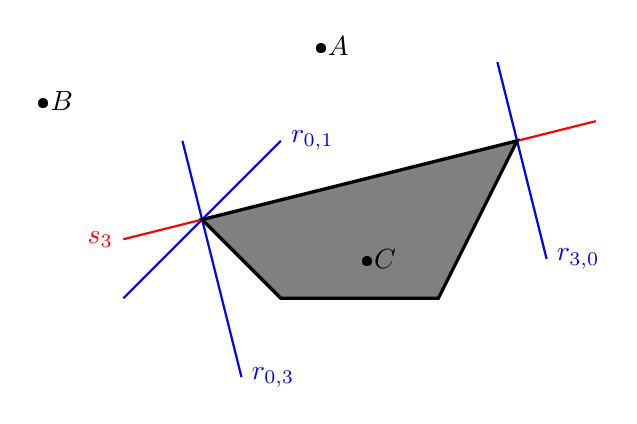
\begin{tikzpicture} 
[cube/.style={very thick,black}, 			
grid/.style={very thin,gray},
cube_hidden/.style={very thick,dashed},
polygon/.style={very thick, black},
axis/.style={-,blue,thick},
point/.style={very thick,black}]
	
%draw a grid in the x-y plane 	
% \foreach \x in {-0.5,0,...,3.0} 		
% \foreach \y in {-0.5,0,...,3.0}
% { 			
% \draw[grid] (\x,-0.5) -- (\x,3.0); 			
% \draw[grid] (-0.5,\y) -- (3.0,\y); 		
% }

%draw the XYZ axes 	
% \draw[axis,red] (3.0,3.0,0) -- (3.5,3.0,0) node[anchor=west,color=red]{$x$}; 	
% \draw[axis,red] (3.0,3.0,0) -- (3.0,3.5,0) node[anchor=west,color=red]{$y$}; 	
% \draw[axis,red] (3.0,3.0,0) -- (3.0,3.0,0.5) node[anchor=west,color=red]{$z$};

%draw the ABC axes 	
% \draw[axis] (0,0,0) -- (3,0,0) node[anchor=west]{$a$}; 	
% \draw[axis] (0,0,0) -- (0,3,0) node[anchor=west]{$b$}; 	
% \draw[axis] (0,0,0) -- (0,0,3) node[anchor=west]{$c$};

%draw the front of the cube 
% \draw[cube,fill=gray!100] (2,0,0) -- (2,2,0) -- (2,2,2) -- (2,0,2) -- cycle;

%draw the front-left of the cube 
%\draw[cube,fill=gray!20] (0,2,0) -- (2,2,0) -- (2,2,2) -- (0,2,2) -- cycle;

%draw the top of the cube
%\draw[cube,fill=gray!60] (0,0,2) -- (0,2,2) -- (2,2,2) -- (2,0,2) -- cycle; 

%draw dashed lines to represent hidden edges 	
%\draw[cube_hidden] (0,0,0) -- (2,0,0); 	
%\draw[cube_hidden] (0,0,0) -- (0,2,0); 	
%\draw[cube_hidden] (0,0,0) -- (0,0,2);

%draw the polygon
% \draw[axis,red] (-1.,2.,0) -- (2.,-1.,0) node[anchor=north,color=red]{$s_0$};
% \draw[axis,red] (0.,0.,0) -- (5.,0.,0) node[anchor=west,color=red]{$s_1$};
% \draw[axis,red] (2.75,-.5,0) -- (4.5,3.,0) node[anchor=west,color=red]{$s_2$};
% \draw[axis,red] (5.,2.25,0) -- (-1.,.75,0) node[anchor=east,color=red]{$s_3$};

\draw[axis] (-.25,2.,0) -- (.5,-1.,0) node[anchor=west,color=blue]{$r_{0,3}$};
\draw[axis] (-1.,0.,0) -- (1.,2.,0) node[anchor=west,color=blue]{$r_{0,1}$};
\draw[axis] (3.75,3.,0) -- (4.375,0.5,0) node[anchor=west,color=blue]{$r_{3,0}$};
%\draw[axis,red] (0.,0.,0) -- (4.25,0.,0) node[anchor=west,color=red]{$s_1$};
%\draw[axis,red] (2.75,-.5,0) -- (4.5,3.,0) node[anchor=west,color=red]{$s_2$};
\draw[axis,red] (5.,2.25,0) -- (-1.,.75,0) node[anchor=east,color=red]{$s_3$};
%\draw[axis,red] (-0.5,1.5,0) -- (1.5,-.5,0) node[anchor=east,color=red]{$s_4$};

\draw[point] (2.0,3.2,0) node[anchor=east]{\textbullet $A$};
\draw[point] (-1.5,2.5,0) node[anchor=east]{\textbullet $B$};
%\draw[axis] (2.0,1.0,0) -- (-0.5,-1.5,0) node[anchor=west,color=blue]{$r_{1,0}$};

\draw[polygon,fill=gray!100] (0,1,0) -- (1,0,0) -- (3,0,0) -- (4,2,0) -- cycle;
\draw[point] (2.6,0.5,0) node[anchor=east]{\textbullet $C$};

\end{tikzpicture}}
\caption{Potitioning different cases when calculating distance from point to a 4-vertices convex polygon. \label{fig:convexpolygon}}
\end{figure}

\begin{figure}[!h]
	\centering
	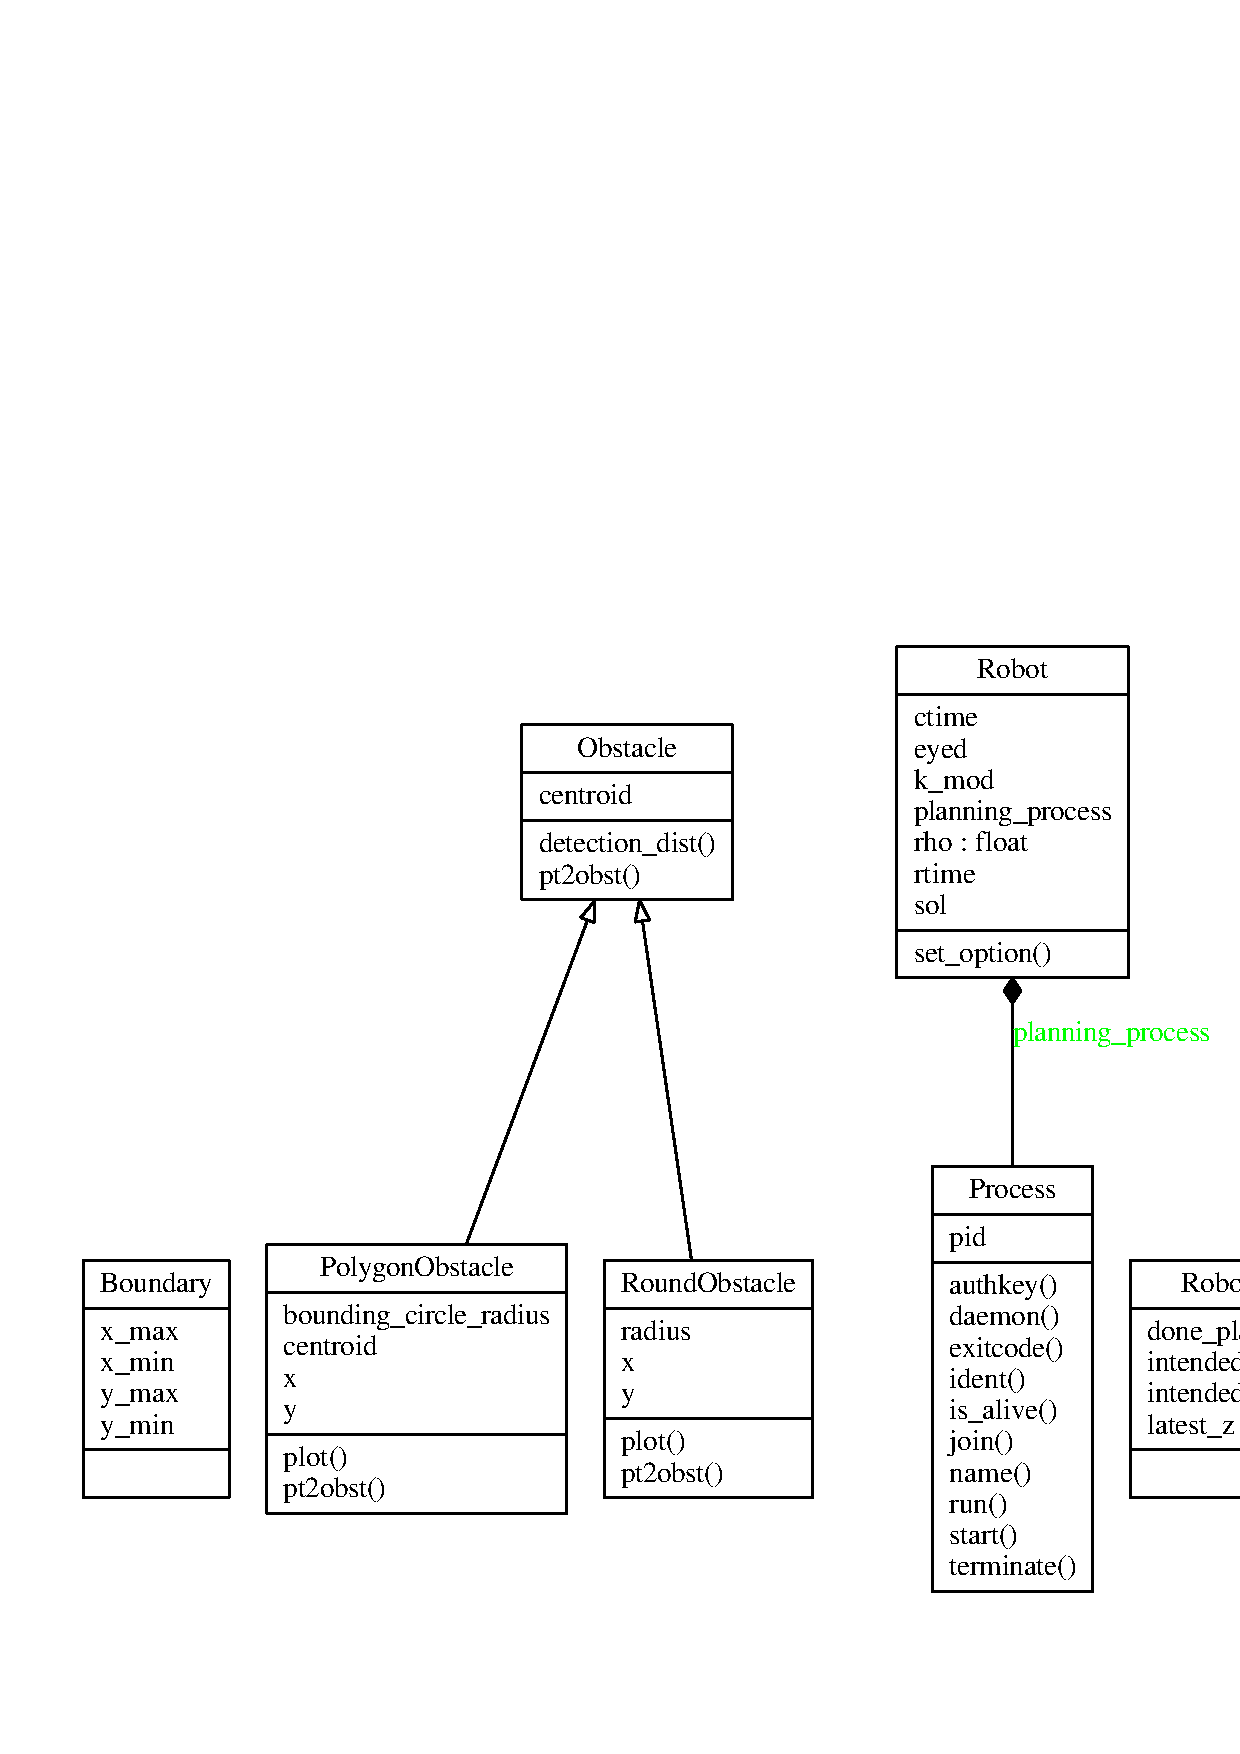
\includegraphics[width=1.\textwidth]{./img/classes_planning.pdf}
	\caption{Class diagram.\label{fig:classesdiagram}}
\end{figure}


\subsection{Multi-robots}

Each robot must be able to access the position of any robot of the fleet. If a robot's position cannot be accessed that means the robot lost its connection with the fleet and will not be considered a conflictual robot by none of the others robots.


Symmetry problem \todo[inline, size=\tiny]{Tc too high no time to avoid another robot involved}

Gilbert-Johnson-Keerthi distance algorithm

\newpage

\section{Class Macther}
\lipsum[1-2]
\subsection{Max-Flow Matcher}
\lipsum[1-3]

\chapter{Incomplete Patches}
\lipsum[1-10]